\documentclass[11pt]{article}

\usepackage[utf8]{inputenc}
\usepackage{fancyhdr}
\usepackage{lastpage}
\usepackage{titlesec}
\usepackage{graphicx}
\usepackage[
    left=0.75in,
    right=0.75in,
    top=1.1in,
    bottom=1in,
]{geometry}

\usepackage{xcolor}
\usepackage{url}
\usepackage{hyperref}
\usepackage{float}

\setlength{\parskip}{3pt}%


\titlespacing{\paragraph}{%
  0pt}{%              left margin
  0.1\baselineskip}{% space before (vertical)
  1em}%   

\begin{document}

\pagestyle{fancy}
\fancyhead{}
\fancyhead[L]{\textbf{Trace-Viz: CS 2640 Final Project}}
\fancyhead[R]{\textbf{Trevor "not a systems guy" DePodesta}}

\fancyfoot{} % clear all footer fields
\fancyfoot[c]{\thepage\ of \pageref{LastPage}}

\noindent\textit{\textbf{Welcome note:} We made it!  My first (and last) systems class is officially over and I'm...sad?  Crazy.  Like we discussed in class, unlike most of the other projects that were presented, this is very much a large-scale engineering project rather than a research project with experiments, results, and rigorous technical evaluations.  As I see it, the system itself (which is being hosted as a live demo for you to play with) speaks largely for itself as an artifact, and this report is mostly supplementary information.  I've really enjoyed working on this, and I've learned a lot---If you're interested, I'd love to explore the idea of expanding on this work and potentially co-authoring something with you this summer/fall!}

\section{Trace-Viz: An Interactive Storage Trace \& Cache Visualizer}
\texttt{trace-viz} is an interactive tool for exploring block I/O traces as a high-performance, interactive heatmap so users can easily and quickly spot access patterns, hotspots, and behavior over time.  It lets users load data from backend-served/uploaded traces, then drill in with pan/zoom, time-window navigation, and region brushing to get focused stats for the visible/selected area.  On top of raw visualization, it supports alternate color encodings, adaptive metrics, cache-simulation overlays with algorithm controls, and an AI-assisted viewport analysis feature that extracts insights from the current view.  In short, it aims to be a single-page analysis tool for turning large, noisy storage traces into actionable visual and quantitative insights.

When I started doing data visualization work, I was taught not to "describe" if there was the option to "show" instead.  In that spirit, the next two pages contain a set of system screenshots, which I've annotated with a set of labels indicating the roughly 18 main features/points of interest the tool contains so far, followed by a brief explanation of each.  Think of it as a visual \texttt{README.md} file for system navigation before you try out the demo.  On that note, the demo is hosted at \href{https://traceviz.netlify.app/}{https://traceviz.netlify.app/}; I ask that you do not share this link with others yet, as the system infrastructure is still relatively hard-coded to expect a 1:1 server:client relationship, and things will start to go wrong if more than one host attempts to interact with the REST API at once.  I also ask that for the time being, you don't use the 'upload a trace file' feature: the backend is currently being hosted for free on a very tiny server with only 512 MB RAM and 0.1 CPUs.  Amazingly, that's enough to run the system, but probably not enough compute to do the real-time analysis of a massive trace file you would likely test.  If you \textit{really} want to test the feature, you can download the \texttt{test\_mini\_trace.csv} file from the monorepo root and use that; it's just a shortened section of the sample cloudPhysicsIO trace.  Because I'm using a free hosting tier for the backend, it will spin down after 5 minutes of inactivity.  Allow up to 50 seconds the first time you access the tool for the trace to load (i.e. for the server to physically start) accordingly.  Some of the features were just implemented in the last few days, and haven't been as rigorously tested---if anything breaks, freezes, appears, or doesn't disappear, a simple refresh should resolve the situation.

\begin{figure}
    \centering
    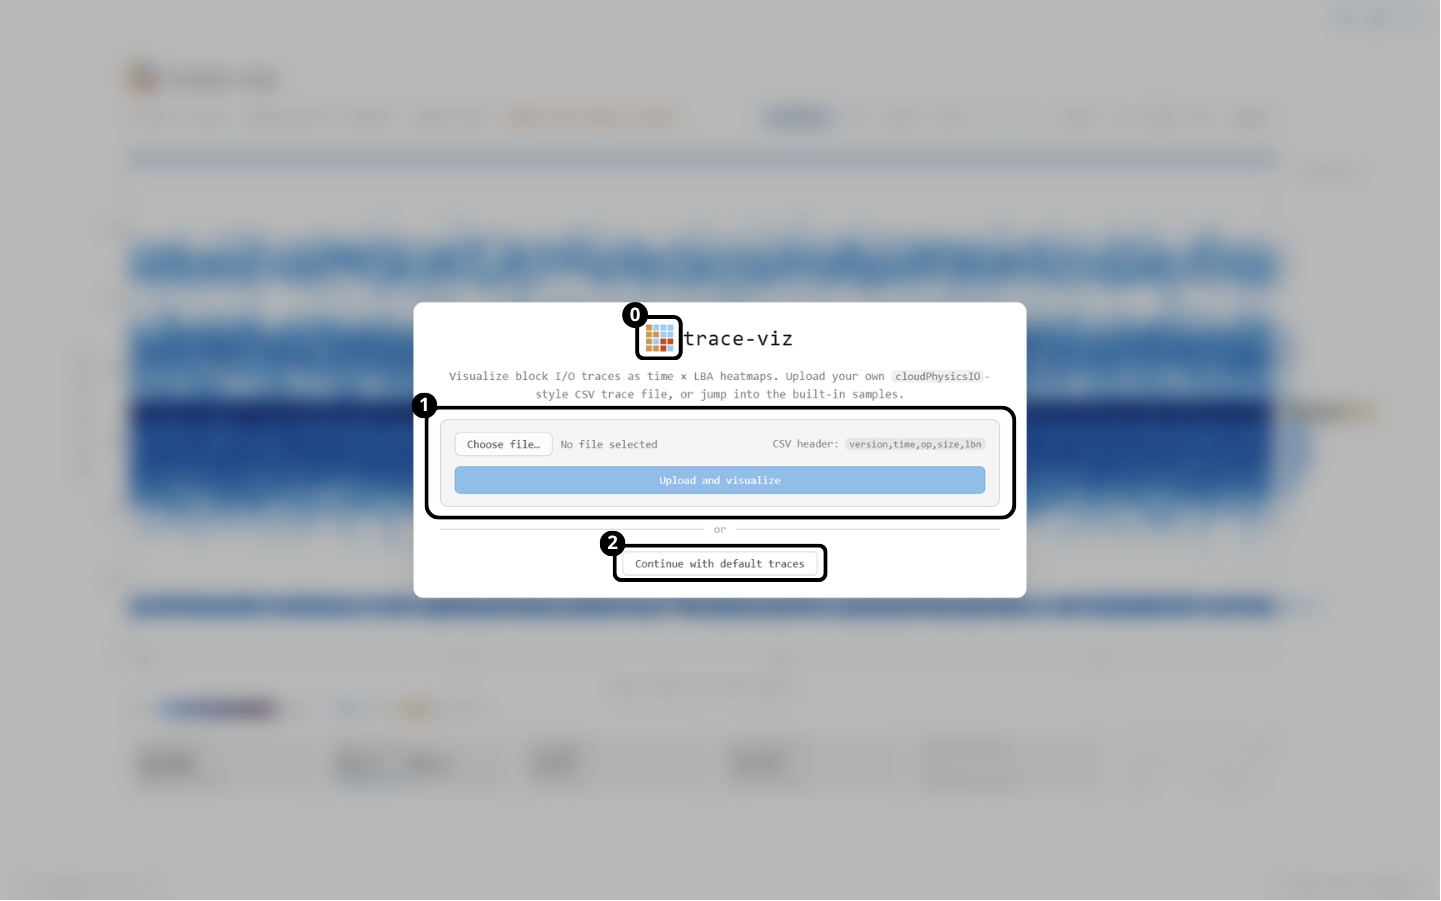
\includegraphics[width=1\linewidth]{trace-viz.png}
    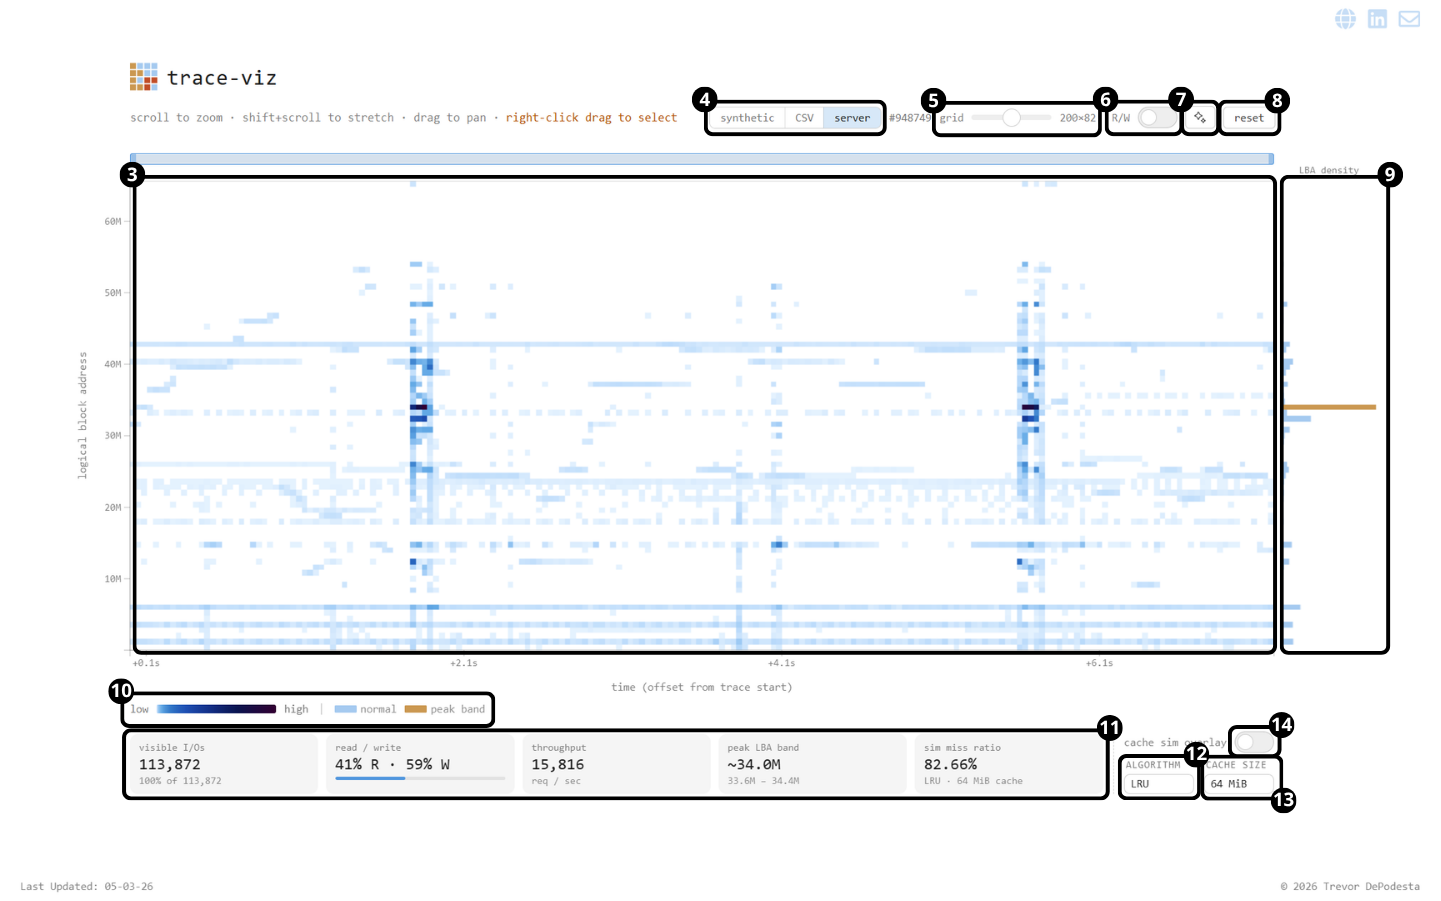
\includegraphics[width=1\linewidth]{trace-viz (1).png}   
\end{figure}

\begin{figure}
    \centering
    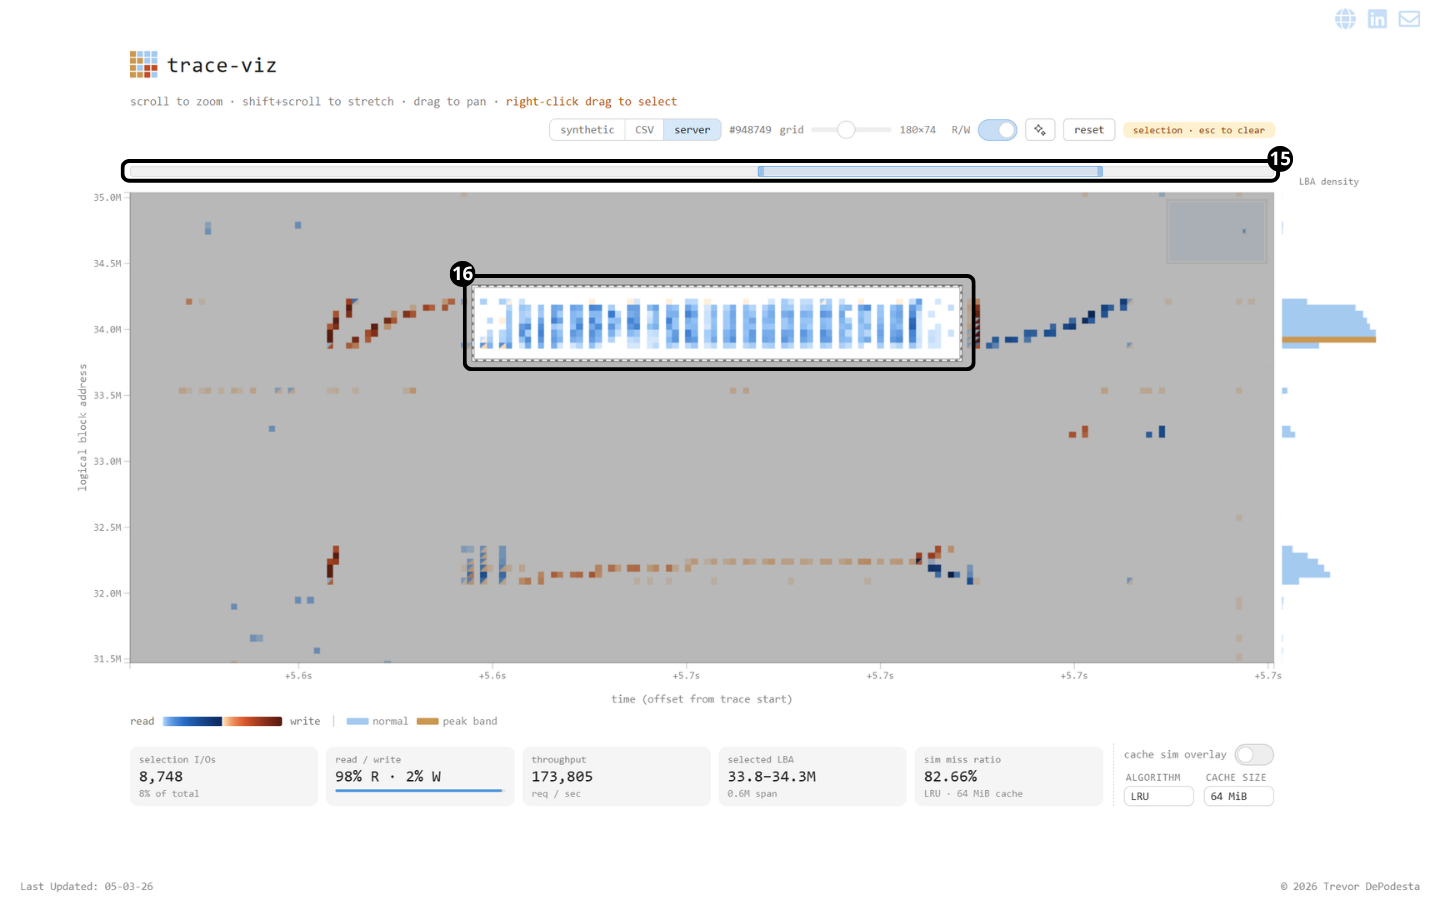
\includegraphics[width=1\linewidth]{trace-viz (2).png}
    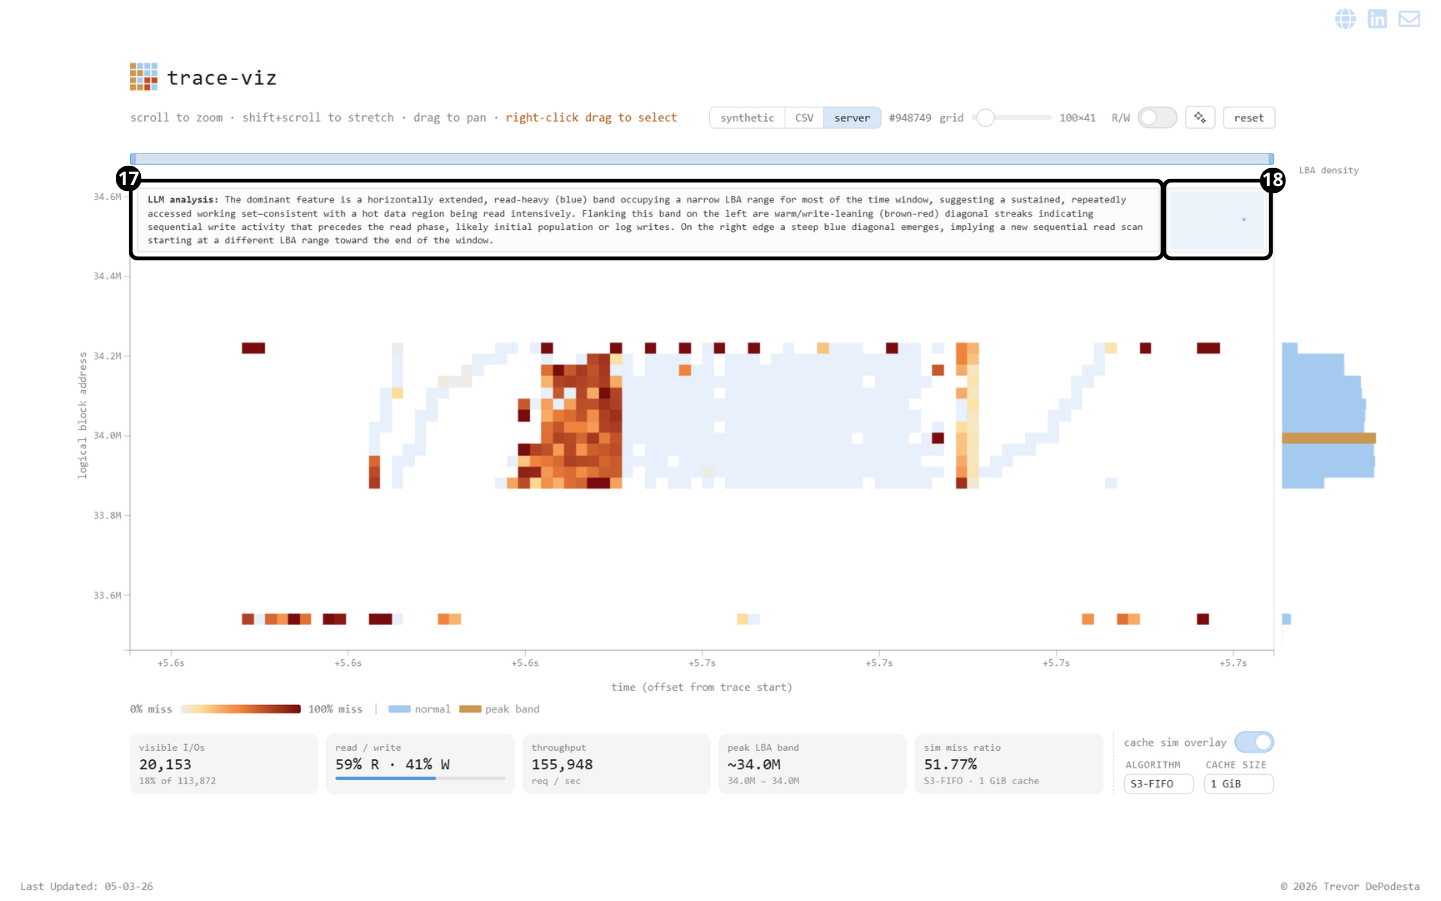
\includegraphics[width=1\linewidth]{trace-viz (3).png}   
\end{figure}

\section{Visual System Walkthrough}
The following descriptions refer to the labels on the four system screenshots.  Item 0 is the favicon logo for the project/demo site.  If you look closely, it's a mini heatmap that hides the lowercase letters "tr" for \textbf{tr}ace-viz!

\begin{enumerate}
    \item \textbf{File Upload:} On startup, users get a welcome dialog that introduces the app and offers local file selection for trace upload.  On success, the app switches to server-backend mode and refreshes the selectable trace list automatically.
    \item \textbf{Default Traces:} By default, the \texttt{cloudPhysicsIO.csv} trace is bundled with the system backend, and lets users explore the tool through an example trace without needing to provide one of their own.  This is dynamically built to allow $n$ number of pre-shipped traces to choose from in the future.
    \item \textbf{Interactive Heatmap:} This is the main view of \texttt{trace-viz}.  The main interactive heatmap maps I/O behavior into a time-by-LBA density view, binning and coloring operations to reveal hotspots and access structure at scale.  Users can scroll to zoom, drag to pan, and shift + scroll to zoom along the x (time) axis only.
    \item \textbf{Demo Data Modes:} For demo purposes only, I've configured the system to work in three different modes: synthetic, CSV, and server.  Server is the main, feature complete implementation, but in environments where a backend is unavailable, the other two options remain as backups.  CSV switches to read trace data from a local copy of the example trace file, bundled into the frontend at build time.  Synthetic generates a synthetic I/O trace.  In both cases, certain features (e.g. cache simulations) are disabled and grayed out, but the main heatmap and associated interactions will continue to function without a network connection.
    \item \textbf{Grid Density:} Depending on (1) one's browser's available memory, or (2) the scale of pattern they're hoping to identify, the tool allows for a dynamic grid density to be set on a sliding scale.  This ranges from $80\times32$ to $320\times132$.
    \item \textbf{Read/Write Toggle:} By default, the heatmap is monochromatic, with relative luminosity encoding density, since each cell is a bin of I/O operations.  By turning on this toggle however, you can enter a split color encoding, where read is blue and write is red.  Cells that contain all read or all write operations abide by the normal rules, and cells with both get split into two diagonal triangles, where the luminosity of each implicitly encodes the respective ratio.
    \item \textbf{LLM Analysis:} Surprise!  I know you didn't think I'd be able to integrate something like this by the end of the semester---lots of 3am debugging sessions made it possible.  Pressing this button sends a (cleanly rendered) snapshot of the current viewport to the server for LLM-extracted insights.  While waiting for the tool call response, the entire UI is grayed out and a CSS loading animation plays.
    \item \textbf{Reset View:} Pressing this button resets the viewport to be fully zoomed out and back on a (0, 0) offset.  All other visual changes (e.g. the read/write toggle) are unaffected.
    \item \textbf{LBA Density Histogram:} To the side of the main heatmap I've included a marginal histogram that renders the relative densities of each rendered LBA band, with the peak band highlighted in orange.  This makes it easy to the distribution of I/Os on the disk at a glance.  In the future I hope to make these bands selectable, allowing a user to highlight a horizontal slice of the heatmap and get filtered metadata.
    \item \textbf{Legend:} This legend remains constantly positioned, and is updated depending on what mode a user is in.  Looking at read/write distributions or cache hit/miss overlays will automatically update the legend.
    \item \textbf{Metadata Cards:} A set of four or five cards display the following statistics at a glance: visible I/Os, read/write ratio, throughput, peak LBA band, and (when a cache eviction algorithm is selected) simulation miss ratio. These statistics provide a snapshot of the viewport, not the trace, meaning they will update live as a user zooms, pans, or selects.
    \item \textbf{Eviction Algorithm:} This dropdown menu allows a user to select an eviction algorithm to use for the cache simulation.  Currently supports FIFO, LRU, Clock, SIEVE, and S3-FIFO.
    \item \textbf{Cache Size:} This dropdown menu allows a user to select the size of their simulated cache, ranging from 1 MiB to 1 GiB.
    \item \textbf{Cacher Simulation Toggle:} This toggle allows users to run and render a simulation of how their configured cache would perform on the visualized trace file.  Hits/misses are visualized through an alternate color encoding, inheriting the same density coloring logic.  This means that it is currently impossible to see both read/writes and cache hit/misses at the same time, since they use the same encoding channel.
    \item \textbf{Time Navigation Bar:} A scrubber bar at the top of the heatmap allows users to quickly "stretch" or "squeeze" the time axis of their view, to expand or minimize details.  Dragging either side of the scrubber thumb will adjust the viewport aspect ratio, while moving the entire thing to the left or right will horizontally transform the current view.  This is particularly useful as a method of fine-grain navigation control when exploring a specific band of LBAs.
    \item \textbf{Selection Window:} By right clicking and dragging, a user can select a rectangular window of the viewport for isolated inspection, graying out the rest of the view.  The statistics in the metadata cards will update to reflect the snapshot of the new selection.
    \item \textbf{LLM Response:} After triggering an LLM analysis, the response is presented as a slightly translucent dialogue box at the top of the heatmap.  There is currently no built-in dismissal mechanism save for initiating another analysis query.
    \item \textbf{Minimap:} The minimap renders a user's viewport in miniature with respect to the full potential viewport, grounding their view in context.  This is especially useful for seeing how early/late into the trace one has zoomed in.
\end{enumerate}

\section{Performance Optimizations}
A big challenge in both the project proposal and project midterm check-in was performance.  The existing workflow of generating static mat-plot-lib scatterplots of trace data works because they're static.  Once they need to be re-rendered after any user interaction (e.g. zooming/panning), the rendering itself becomes the principal limitation.  I have implemented the following list of performance optimizations to mitigate this issue, such that now the server-side processing is the limiting bottleneck.  Some of them are fairly naive and trivial, while others singlehandedly resulted in major performance impacts.

\subsection{Frontend}
\begin{itemize}
    \item Canvas-first rendering: the heatmap is rendered on a single \texttt{<canvas/>} with SVG only used for interaction overlays, avoiding huge numbers of DOM nodes
    \item Server aggregate tile cache reuse: the frontend stores the last aggregate tile and reuses it when the current viewport is still covered at acceptable effective resolution.  I.e. small pans/zooms can skip a round-trip and reduce visible redraw latency.
    \item Predictive over-fetching: aggregate requests include padding around the visible time/LBA window, giving the UI "buffer" data for near-future navigation so subsequent small movements hit cache
    \item Aggregate request deduping by key: A request key (trace id + bounds + grid + sim parameters) is tracked to avoid sending duplicate in-flight requests, preventing bursty interaction.
    \item Short-delay scheduling to coalesce interaction bursts: aggregate fetch triggering is delayed very slightly ($\sim$16ms) so rapid input events collapse into fewer requests.
    \item Adaptive grid resolution + hard caps: grid dimensions are constrained with an upper bound, guaranteeing that at any given time the maximum number of cells being rendered is capped at 42,240.
    \item Precomputed cell edge arrays per draw: pixel boundaries for grid edges are computed once and reused in inner loops, reducing repeated coordinate math.
    \item Render suppression for stats updates: only push new stat values to React state when they meaningfully differ (i.e. don't round to the same displayed value) to limit VDOM updates.
    \item Heavy use of React refs for hot-path state access: mirror more frequently read mutable values into refs to avoid rebinding on state change.
    \item Memoization of expensive derived values: especially useful around synthetic dataset generation and bundle composition.
\end{itemize}

\subsection{Backend}
\begin{itemize}
    \item Columnar NumPy materialization + in-process trace cache: parsed trace rows are transformed into NumPy arrays once and cached in memory per trace, removing Python dict iteration on every aggregate request.
    \item Stable time sort during preprocessing: data is sorted by time once, enabling fast window slicing later and making binary-search windowing possible.
    \item Binary search viewport narrowing: requests first compute \texttt{[lo, hi]} indices for the time window via binary search and then only operate on that slice (O(n) $\rightarrow$ O(log n)).
    \item Vectorized 2D binning: bin coordinates are computed as arrays with flattened indices counted in vectorized form, replacing Python loops with compiled NumPy operations.
    \item Single-pass multi-metric accumulation: the same computed bin indices are reused for total, read, and miss-count maps.
    \item Pre-normalized ingestation: CSV rows are parsed into typed fields at ingest time.
    \item Oracle binary trace generation for simulation: cache simulation uses a packed binary trace format (but you know this, you wrote libCacheSim.  By the way, it has so installation problems with WSL2, but we can talk about that another time.  For now I'm just using a Linux vm).
    \item Oracle file reuse checks: backend verifies expected record count/size and reuses existing oracle files when valid.
    \item Two-level simulation caching: simulation outputs are memoized in memory and persisted on disk (.npz) keyed by algo + trace + size.  Repeated requests with the same parameters can return without rerunning simulations.
    \item Preallocated simulation result arrays: self explanatory.
    \item Payload size caps for uploads/analyze endpoints: same.
\end{itemize}

\section{LLM Analysis is Really Hard}
I tried so.  Many.  Different.  Techniques.  In the end, it was clear I wasn't going to be able to get the visual annotations working before this was due, so I settled on just the natural language analysis for now.  To commemorate my struggles, I present the gallery of failed computational annotations:

\vspace{2em}

\begin{figure}[H]
    \centering
    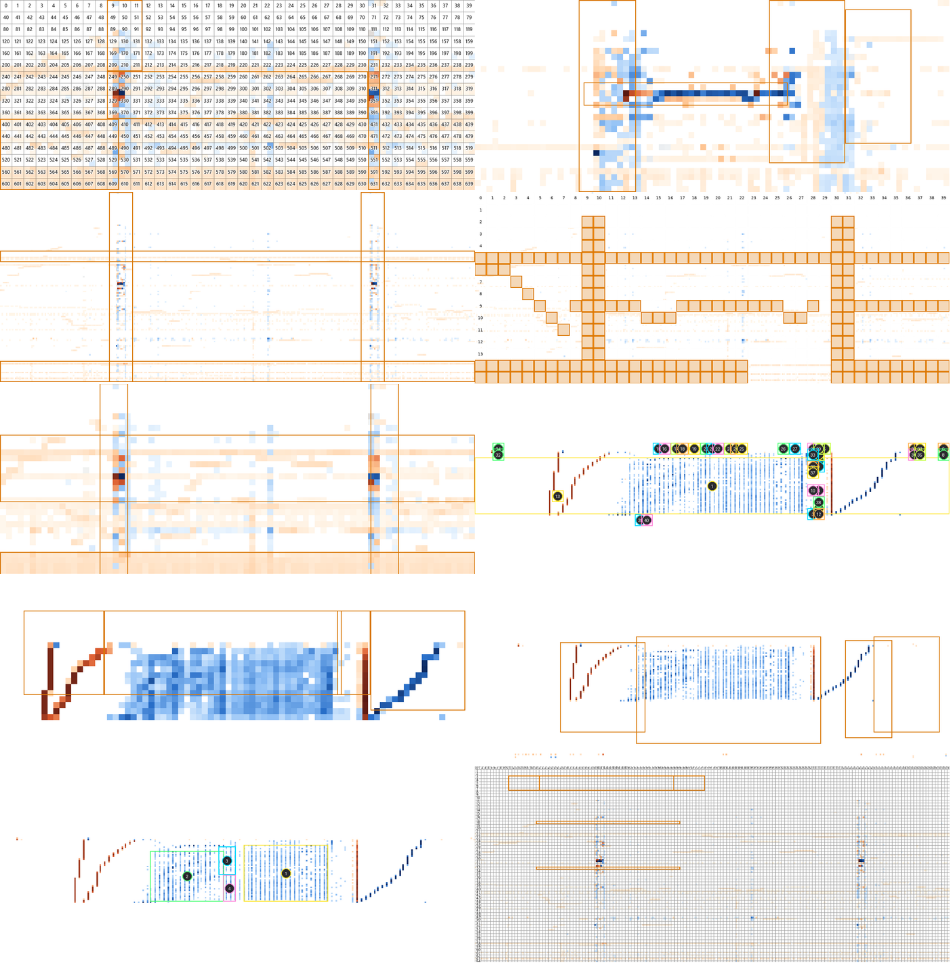
\includegraphics[width=1\linewidth]{trace-viz (4).png}
\end{figure}

\end{document}
